\documentclass[a4paper]{jsarticle}

% 余白
\usepackage[top=20truemm, bottom=25truemm, left=22truemm, right=22truemm]{geometry}
% 数式
\usepackage{amsmath, amssymb}
\usepackage{ascmac}
\usepackage{mathtools}
\mathtoolsset{showonlyrefs,showmanualtags} 	 % 相互参照した式のみに番号を振る
% 画像
\usepackage[dvipdfmx]{graphicx}
\usepackage[subrefformat=parens]{subcaption}
\captionsetup{compatibility=false}
% ハイパーリンク
\usepackage[dvipdfmx]{hyperref}
\usepackage{pxjahyper}

% コマンド定義
\def\vec#1{\mbox{\boldmath $#1$}}
\newcommand{\dif}[2]{\frac{{\rm d} #1}{{\rm d} #2}}
\newcommand{\pdif}[2]{\frac{\partial #1}{\partial #2}}
\newcommand{\ddif}{{\rm d}}

\title{\S 35.\ オイラーの角}

\begin{document}
\maketitle

今までに見てきたように、剛体の記述をするためには、
慣性系から見た慣性中心の座標(3自由度)と、
慣性系の座標軸からどれだけ回転しているか(3自由度)の、合計6自由度が必要である。
前者の3自由度の決め方は、特に述べる必要はないだろう(普通に定めれば良い)。
ここで問題にするのは後者の回転に関する自由度の決め方である。
回転角は様々な方法で定めることができるが、ここでは多くの場合で便利である
\textbf{オイラー(の)角}を用いる。

運動系の軸が慣性系の軸からどれだけ回転しているかを見るために、
常に運動系の原点と慣性系の原点が一致するように平行移動させてから考えても良い。
以降はそのようにした後の、慣性系$(X, Y, Z)$、
運動系$(x_1, x_2, x_3)$を考えることにする。
すると、まず$Z$軸と$x_3$軸のなす角$\theta (0 \le \theta \le \pi)$を
定めることができる。

次に、$\theta \ne 0, \pi$のとき、$XY$平面と$x_1 x_2$平面は同じでないから、
ある交線$ON$(平面が共有する直線)を持つことになる。
この交線$ON$は$XY$平面内にあるから、$Z$軸に垂直であり、
また$x_1x_2$平面内にあるから$x_3$軸にも垂直である。
したがって$ON$の正の方向を、$Z$軸から$x_3$軸に回した方向$[\vec{e}_{Z} \vec{e}_{x_3}]$
と定めることができる。
その上で$X$軸と$ON$がなす角を$\phi (0 \le \phi < 2\pi)$とし、
$ON$と$x_1$軸がなす角を$\psi (0 \le \psi < 2\pi)$と定める。
もし$\theta = 0, \pi$であれば、$X$軸と$x_1$軸のなす角を$\phi$とし、
$\psi=0$となることになる。

ここで$\theta$だけが$0 \le \theta \le \pi$の範囲に制限されるのは、
最初$\theta$を定める際には、基準になる方向がなく、単純に$Z$軸と$x_3$軸がなす角しか
分からないからである。
しかし、$\phi$は右ねじの方向が$Z$軸方向になるように、
$\psi$は右ねじの方向が$x_3$軸方向になるように定めるため、
角度が$0$から$2\pi$まで動くことになる。

\setcounter{figure}{46}
\begin{figure}[h]
	\begin{center}
		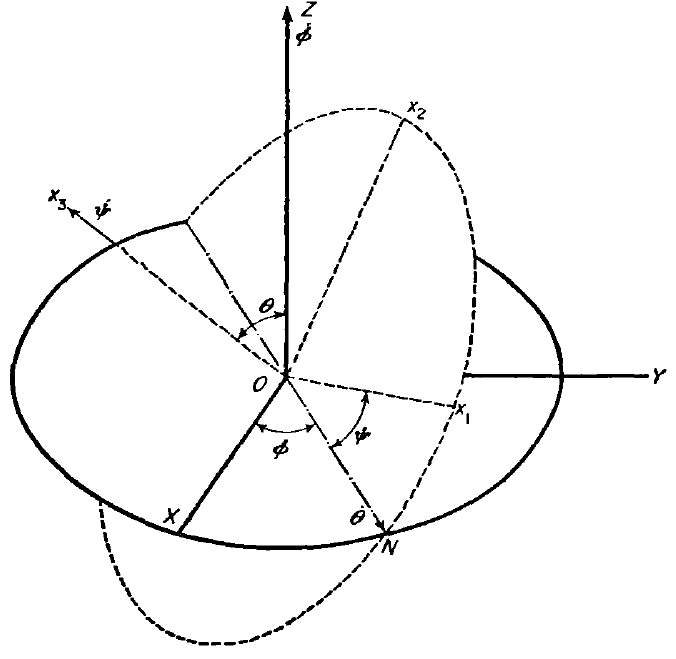
\includegraphics[width=0.5\linewidth]{fig/47.png}
	\end{center}
	\caption{}
	\label{fig:angle}
\end{figure}

角度が分かったあとに、この回転を再現する方法は色々あるが、一例を示しておく。
まず最初$x_1, x_2, x_3$軸はそれぞれ$X, Y, Z$軸と一致しているとする。
その状態から、$Z$軸周りに$x_1$軸を$\phi$だけ回転させる。
その後に$x_1(ON)$軸周りに$x_3$軸を$\theta$だけ回転させる。
最後に$x_3$軸周りに$x_1$軸を$\psi$だけ回転させる。
このようにすることで、再現したい状態を再現することができる。
なぜなら、まず$x_2$軸は$[\vec{e}_{x_3} \vec{e}_{x_1}]$と方向が一致するように
作れば一意であるから、気にする必要はない。
次に$x_1$軸に関しては、最終的に$ON$と$x_1$軸のなす角を$\psi$にしたいが、
$ON$と$x_1$軸は共に$x_3$軸に垂直な平面内にあるため、
最後に$x_1$軸を$ON$から$\psi$回転させれば良いことが分かる。
そのために$ON$の位置に$x_1$軸を動かす必要があるが、
初期の$x_1(X)$軸と$ON$は共に$Z$軸に垂直な平面内にあり、なす角が$\psi$であるから、
最初の回転で$x_1$軸が$ON$と一致するようになる。
2つ目は$x_1$軸周りに回転させるため、動かない。
したがって、この順番で回せば、作りたい$x_1$軸を作ることができることが分かる。
また、$x_3$軸であるが、最初の回転では$Z$軸と一致している。
次に$X$軸周りに$x_3$軸を回転したが、
最後は$x_3$軸は(もちろん$Z$軸も)動かさないから、
結局2つ目で$\theta$だけ回転させたことしか、結果に効いてこない。
これで再現したい状態を再現できた。

\begin{screen}
	\underline{補足}

	同じ再現を、$x_1(X)$軸周り、$Z$軸周り、$x_3$軸周りにやることでもできる。

	この再現方法から$x_3$軸の$X, Y, Z$軸に関する($Z$軸から見た)天頂角、
	($X$軸から見た)方位角、$Z$軸の$x_1, x_2, x_3$軸に関する($x_3$軸から見た)天頂角、
	($X$軸から見た)方位角をそれぞれ知ることができる。
	まず$x_3$軸に関しては、$Z$軸からは$\theta$だけ回転しているから、
	天頂角は$\theta$となる。
	また、それは$X$軸周りの回転、つまり$Y$軸から$Z$軸方向に回す回転だから、
	$X$軸となす角は$-\pi/2$になっている。
	その状態で$Z$軸周り、つまり$X$軸から$Y$軸方向に$\phi$回すから、
	方位角は$\phi - \pi/2$になっている
	(そのあとの$x_3$軸周りの回転では、$x_3$は固定されている)。

	$Z$軸に関しては、最初は$x_3$軸と同じ効果が出るから、天頂角は$\theta$になる。
	しかし、方位角に関しては$Z$軸から見れば、$x_3$軸から$x_2$軸に向かう方向に
	$\theta$回されることになるから、$x_1$軸となす角は$\pi/2$になっている。
	次の回転は$Z$軸周りだから効いてこず、その次の回転が$X_3$軸周り、
	つまり$x_1$軸から$x_2$軸方向への回転で、$Z$軸では逆になるため、
	$-\psi$回転することになる。
	したがって最終的な方位角は$\pi/2 - \psi$となる。
\end{screen}

ここまでの議論を踏まえて、このオイラー角から剛体の
角速度ベクトル$\vec{\Omega}$を求める。
後に補足で与えるが、微小回転をベクトルの外積で与える場合には、
その微小回転を代表するベクトル同士は足して、1つのベクトルとして作用させることができる。
そこで、微小時間$\ddif t$の間に各$\theta, \phi, \psi$が微小量
$\ddif \theta, \ddif \phi, \ddif \psi$だけ変化することを考える。
これら微小変化をベクトル$\ddif \vec{\theta}, \ddif \vec{\phi}, \ddif \vec{\psi}$と
書くと、それぞれその定義の仕方から、$ON$、$Z$軸、$x_3$軸方向を向いている。
今求めたいのは、運動系$(x_1, x_2, x_3)$での角速度$\vec{\Omega}$の表示であるから、
それらの微小ベクトルを、$x_1, x_2, x_3$軸に分割することを考える。
以降微小角度ベクトル$\ddif \vec{\alpha}$の$x_i$軸への投影を
$\ddif \alpha_i$と書くことにする。

まず$\ddif \vec{\theta}$について考えると、これは$x_3$軸には垂直であるから、
その方向には成分を持っていない。また$x_3$軸周りに$x_1$軸を$ON$から
角度$\psi$だけ回転させているから、
\begin{align}
	&\ddif \theta_1 = \ddif \theta \cos \psi \\
	&\ddif \theta_2 = -\ddif \theta \sin \psi \\
	&\ddif \theta_3 = 0
\end{align}
と書ける。
次に$\ddif \vec{\phi}$に関しては、$Z$軸の$(x_1, x_2, x_3)$でみたときの天頂角、
方位角から
\begin{align}
	&\ddif \phi_1 = \ddif \phi \sin \theta \sin \psi \\
	&\ddif \phi_2 = \ddif \phi \sin \theta \cos \psi \\
	&\ddif \phi_3 = \ddif \phi \cos \theta
\end{align}
となる。
最後に$\ddif \vec{\psi}$については、
明らかに$x_3$軸方向についてしか成分を持っていない。

以上から、結局全微小回転ベクトルを$\ddif \vec{\alpha}$とすると、その成分は
\begin{align}
	&\ddif \alpha_1 = \ddif \phi \sin \theta \sin \psi
	+ \ddif \theta \cos \psi \\
	&\ddif \alpha_2 = \ddif \phi \sin \theta \cos \psi
	- \ddif \theta \sin \psi  \\
	&\ddif \alpha_3 = \ddif \phi \cos \theta + \ddif \psi
\end{align}
と書けることが分かる。
したがって、角速度$\vec{\Omega}$の各成分は
\begin{align}
	&\Omega_1 = \dif{\alpha_1}{t} = \dif{\phi}{t} \sin \theta \sin \psi
	+ \dif{\theta}{t} \cos \psi \\
	&\Omega_2 = \dif{\alpha_2}{t} = \dif{\phi}{t} \sin \theta \cos \psi
	- \dif{\theta}{t} \sin \psi \\
	&\Omega_3 = \dif{\alpha_3}{t} = \dif{\phi}{t} \cos \theta + \dif{\psi}{t}
\end{align}
である。

\begin{screen}
	\underline{補足}

	ここで少し微小回転についての補足をしておく。
	まず$z$軸周りで$\vec{r} = {}^t\!(x, y, z)$を角度$\phi$だけ回転させることを考える。
	そのとき回転行列
	\begin{align}
		R = \left( 
			\begin{array}{ccc}
				\cos \phi & -\sin \phi & 0 \\
				\sin \phi & \cos \phi & 0 \\
				0 & 0 & 1
			\end{array}
		 \right)
	\end{align}
	を用いると、移動後の位置ベクトル$\vec{r}^{\prime}$は
	\begin{align}
		\vec{r}^{\prime} = R \vec{r}
	\end{align}
	と書ける。
	ここで回転角度$\phi$が微小量$\ddif \phi$ならば、$R$は
	\begin{align}
		R = \left( 
			\begin{array}{ccc}
				1 & -\ddif \phi & 0 \\
				\ddif \phi & 1 & 0 \\
				0 & 0 & 1
			\end{array}
		 \right) + O(\ddif \phi^2)
	\end{align}
	と書き直せる。
	このとき$\vec{r}$の変化量$\ddif \vec{r}$は
	\begin{align}
		\ddif \vec{r} &= \vec{r}^{\prime} - \vec{r} \\
		&= (R - I) \vec{r} \\
		&= \left( 
			\begin{array}{ccc}
				0 & -\ddif \phi & 0 \\
				\ddif \phi & 0 & 0 \\
				0 & 0 & 0
			\end{array}
			\right) \left(
				\begin{array}{c}
					x \\ y \\ z
				\end{array}
			\right) + O(\ddif \phi^2) \\
		&= \left(
			\begin{array}{c}
				-y \ddif \phi \\ x \ddif \phi \\ 0
			\end{array}
		\right) + O(\ddif \phi^2)
	\end{align}
	となる。
	これは
	微小回転ベクトル$\ddif \vec{\phi} = {}^t\!(0, 0, \ddif \phi)$を用いれば、
	\begin{align}
		\ddif \vec{\phi} \times \vec{r} = \left(
			\begin{array}{c}
				0 \\ 0 \\ \ddif \phi
			\end{array}
		\right) \times \left(
			\begin{array}{c}
				x \\ y \\ z
			\end{array}
		\right)
	\end{align}
	と微小量の2次以上を無視することで、一致する。
	微小回転はどれもそれを代表させるベクトルを持ってくると、
	回転させたいベクトルとの外積を取ることで、微小変位を求めることができる。
	微小変位はただのベクトルであるから、それらは足し合わせられる。
	つまり、微小回転ベクトル同士は足すことができる。
\end{screen}

ここまでの結果から、$x_1, x_2, x_3$軸を回転主軸に選ぶと、
オイラー角を用いて回転の運動エネルギーを求めることができる。
ここで特に簡単な場合を紹介しておく。
もし剛体が対称こま、つまり$I_1 = I_2 \ne I_3$であれば、$x_3$軸を対称軸に選ぶ。
すると他の2軸は$x_3$軸に垂直な方向で自由に選べるから、
常に$x_1$軸が$ON$に一致するように選ぶことにする。
このとき$\psi = 0$となるから、
\begin{align}
	&\Omega_1 = \dot{\theta} \\
	&\Omega_2 = \dot{\phi} \sin \theta \\
	&\Omega_3 = \dot{\phi} \cos \theta + \dot{\psi}
\end{align}
である。
したがって、
\begin{align}
	T_{\mbox{回転}} &= \frac{1}{2} I_i \Omega_i^2 \\
	&= \frac{I_1}{2} \dot{\theta}^2
	+ \frac{I_2}{2} \left(\dot{\phi} \sin \theta \right)^2
	+ \frac{I_3}{2} \left(\dot{\phi} \cos \theta + \dot{\psi} \right)^2 \\
	&= \frac{I_1}{2} \left(\dot{\theta}^2 + \dot{\phi}^2 \sin^2 \theta \right)
	+ \frac{I_3}{2} \left(\dot{\phi} \cos \theta + \dot{\psi} \right)^2
\end{align}
と書ける。

また33節で見た対称こまの歳差運動をもう1度見直すことにする。
この系では全角運動量$\vec{M}$は保存されるから、方向が一致するように$Z$軸を取る。
また先ほどと同じように$ON$軸と一致するように$x_1$軸を取る。
すると$x_1(ON)$は$Z$軸($\vec{M}$)と垂直だから、
\begin{align}
	M_1 = 0, \quad M_2 = M \sin \theta, \quad M_3 = M \cos \theta
\end{align}
となる。
また先の結果より
\begin{align}
	&M_1 = I_1 \Omega_1 = I_1 \dot{\theta} \\
	&M_2 = I_2 \Omega_2 = I_1 \dot{\phi} \sin \theta \\
	&M_3 = I_3 \Omega_3 = I_3 \left( \dot{\phi} \cos \theta + \dot{\psi} \right)
\end{align}
も成り立つから、
\begin{align}
	\dot{\theta} = 0, \quad \dot{\phi} = \frac{M}{I_1}, \quad
	\Omega_3 = \frac{M}{I_3} \cos \theta
\end{align}
を得る。
1つ目の式は$\theta = {\rm const}$、
つまりこまの対称軸と$\vec{M}$のなす角が変わらないことを意味する。
また2つ目は$Z$軸周りの回転、すなわち歳差運動の角速度を与える。
3つ目はこまの対称軸周りの角速度を与える。

\end{document}